\documentclass{beamer}

\title{Consumers as Tax Auditors}
\author{Joana Naritomi}
\date{\today}

\begin{document}

\frame{\titlepage}

\begin{frame}
\frametitle{Introduction}
\begin{itemize}
\item Access to third-party information and paper trails believed to be critical for administration of modern tax systems.
\item Despite collusion opportunities, how can government still effectively utilize this paper trail generated by economic activities. 
\item We discussed in this class that third-party reporting leads to substantial decrease in evasion  (Gordon \& Li 2009;
Kleven et al. 2016).
\item Therefore extensive margin effect of paper trail is known, but what are the mechanisms and how it avoids collusion among informal transcting parties.  

\end{itemize}
\end{frame}

\begin{frame}
\frametitle{This paper}
\begin{itemize}
    \item This paper exploits quasi-experimental variation and unique administrative data on firms and consumers from an anti-tax evasion program in Sao Paulo, Brazil – Nota Fiscal Paulista (NFP) – that created monetary rewards for consumers to ensure that firms report final sales transactions. 
    \item The program provides tax rebates and
monthly lottery prizes for consumers who ask for receipts, and establishes a direct communication
channel between the tax authority and consumers through an online account system, where consumers can verify receipts reported by firms and can act as whistle-blowers by filing complaints.
\item She constructs unique administrative data on firm-level monthly tax returns, monthly
individual-level data on requested receipts and overall participation in the NFP program, based
on administrative records from the tax authority of the state of Sao Paulo.
\end{itemize}
\end{frame}

\begin{frame}{Empirical Approach}
\begin{itemize}
    \item Compare retail firms vs wholesalers. 
    \item Reported revenue by retail firms increased by 21\% within 4 years of reform. This is likely a lower bound.
    \item Study mechanisms through winners of lottery and volume of firm sales or mass of consumers of a firm. 
\end{itemize}
\end{frame}

\begin{frame}{First Stage}
\begin{figure}
    \centering
    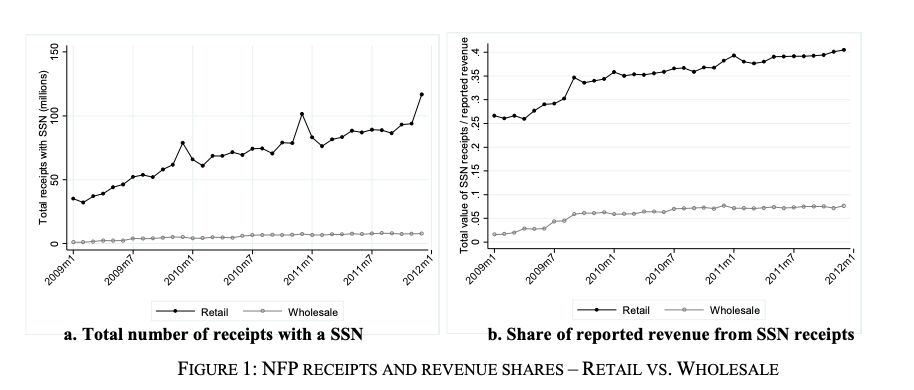
\includegraphics[width=\textwidth]{Paper Presentations/Consumers as Tax Auditors/F1.png}
    \label{fig:enter-label}
\end{figure}
\end{frame}

\begin{frame}{Effect of Reform}
\begin{figure}
    \centering
    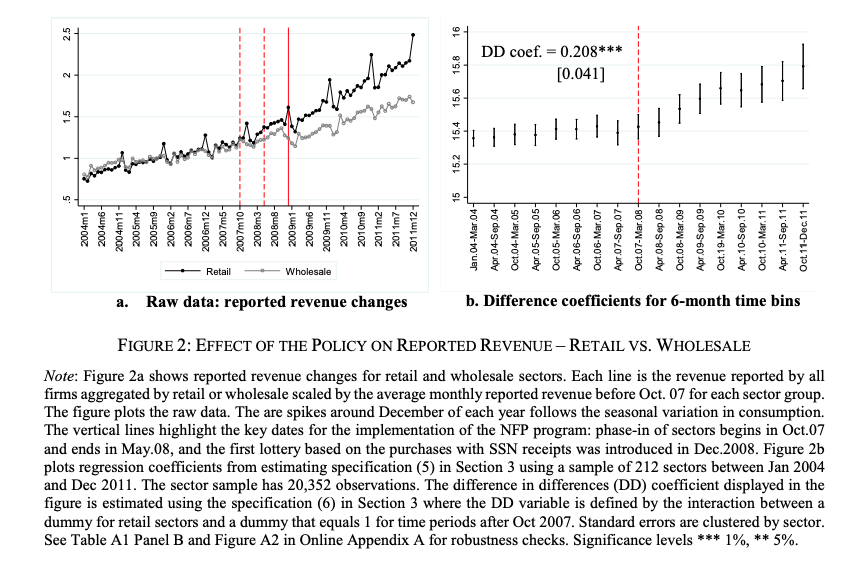
\includegraphics[width=\textwidth]{Paper Presentations/Consumers as Tax Auditors/Impact.png}
    \label{fig:enter-label}
\end{figure}
\end{frame}

\begin{frame}{Who responds to the reform?}
\begin{figure}
    \centering
    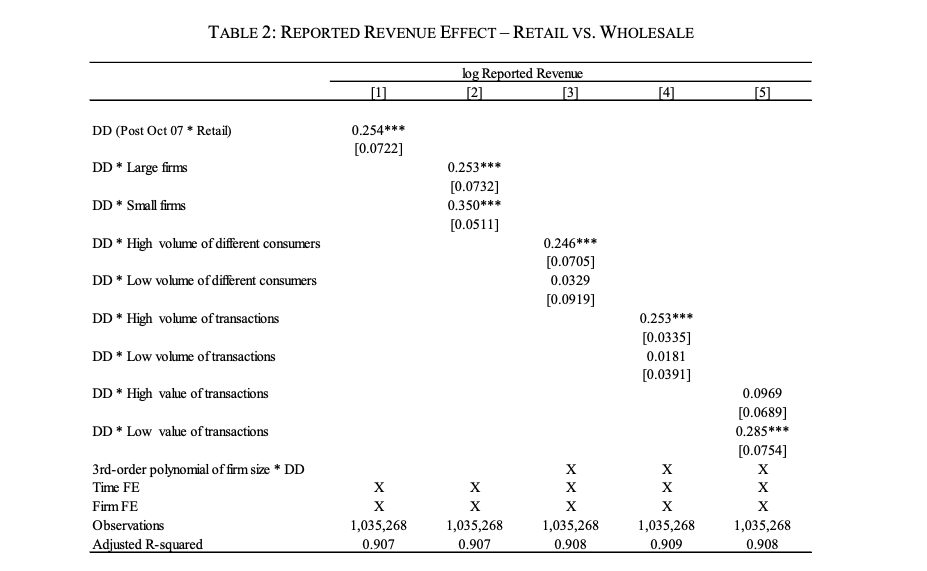
\includegraphics[width=\textwidth]{Paper Presentations/Consumers as Tax Auditors/T1.png}
    \label{fig:enter-label}
\end{figure}
\end{frame}

\begin{frame}{Do they deduct more?}
\begin{figure}
    \centering
    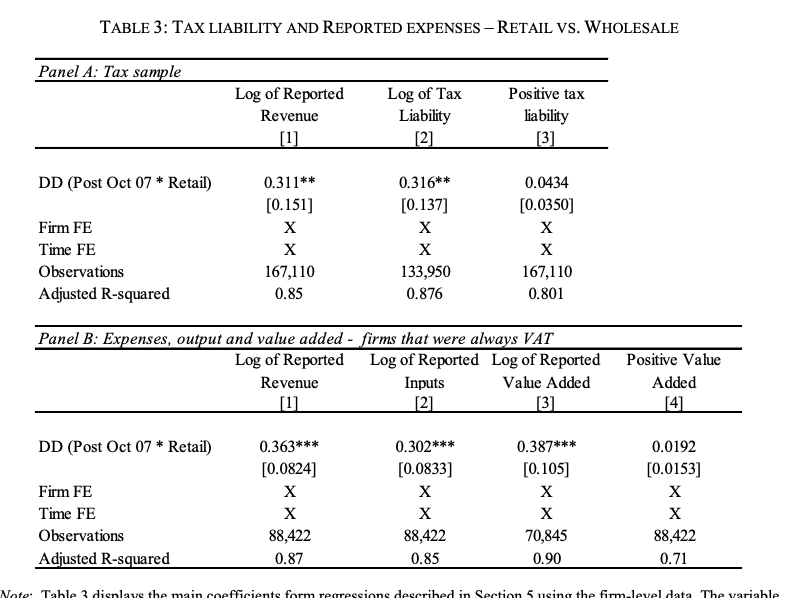
\includegraphics[width=\textwidth]{Paper Presentations/Consumers as Tax Auditors/T2.png}
    \label{fig:enter-label}
\end{figure}
\end{frame}



\begin{frame}
\frametitle{Taxes go up}
\begin{figure}
    \centering
    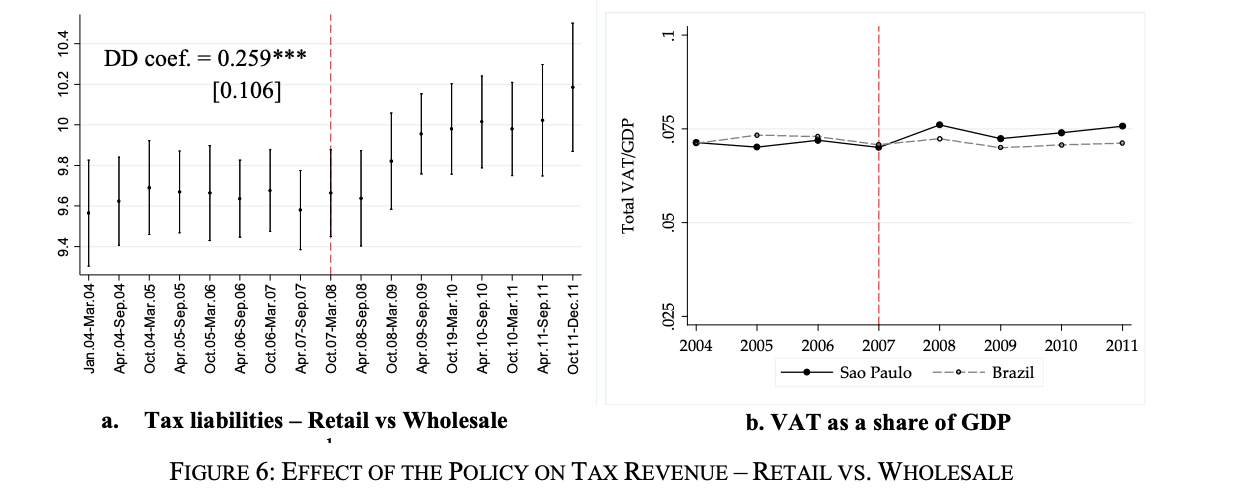
\includegraphics[width=\textwidth]{Paper Presentations/Consumers as Tax Auditors/TEPOLICY.png}
\end{figure}
\end{frame}

\begin{frame}{Effect of Whistle Blowers}
\begin{figure}
    \centering
    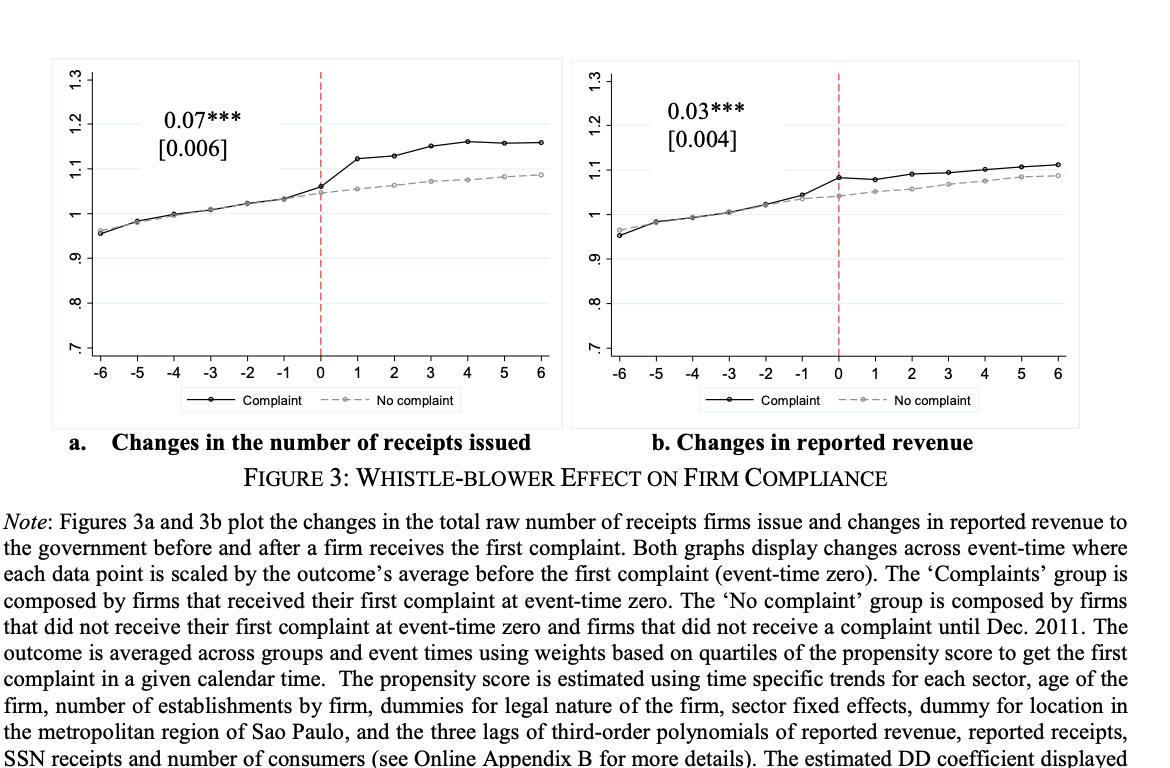
\includegraphics[width=\textwidth]{Paper Presentations/Consumers as Tax Auditors/Whistle Blower.png}
    \label{fig:enter-label}
\end{figure}
\end{frame}

\begin{frame}
\frametitle{Robustness}
\begin{figure}
    \centering
    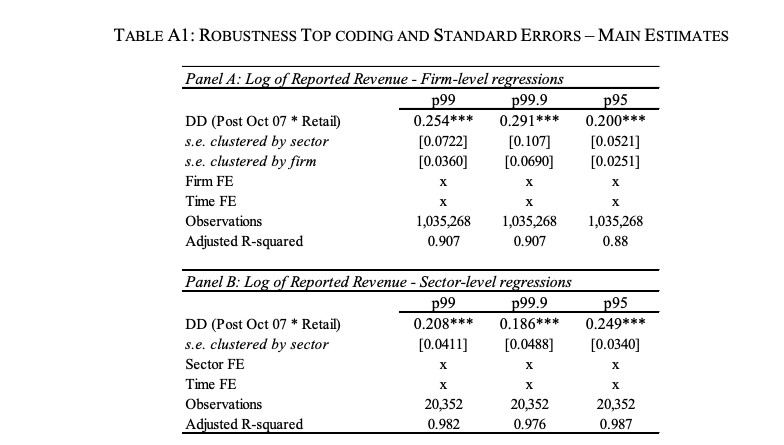
\includegraphics[width=\textwidth]{Paper Presentations/Consumers as Tax Auditors/R1.png}
\end{figure}
\end{frame}


\begin{frame}
\frametitle{Program Participation and Role of Incentives}
\begin{figure}
    \centering
    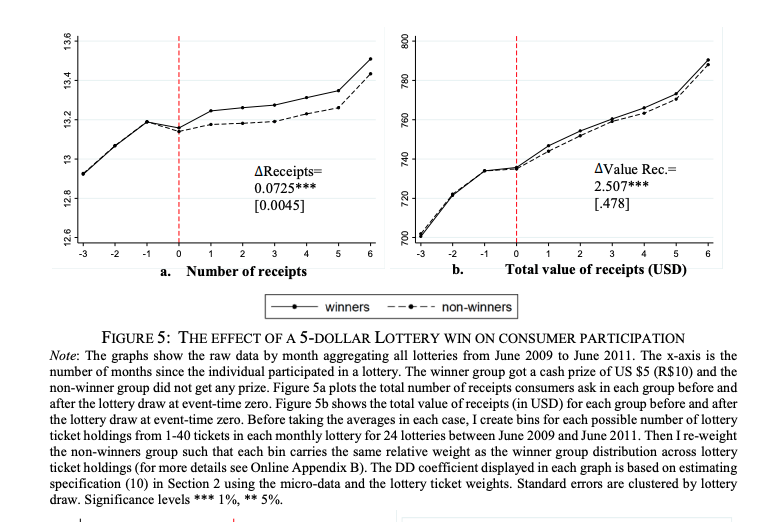
\includegraphics[width=\textwidth]{Paper Presentations/Consumers as Tax Auditors/F5.png}
\end{figure}
\end{frame}

\begin{frame}
\frametitle{Conclusions}
\begin{itemize}
    \item What would be marginal value of public funds? 
    \item Does program pay for itself? tax revenue increased by 9.3\% net of rewards.
    \item However, we do not know the cost of running this program!
\end{itemize}
\end{frame}

\begin{frame}
\frametitle{Broader Implications}
\begin{itemize}
    \item Potential applications in various economic fields.
\end{itemize}
\end{frame}

\begin{frame}
\frametitle{Conclusion}
\begin{itemize}
    \item Main findings and contributions.
    \item Importance in policy analysis.
\end{itemize}
\end{frame}

\begin{frame}
\frametitle{References}
% Add your references here
\end{frame}

\end{document}
